% !TeX root = ../../../main.tex

% Key observations for fig:clinicalVisrDoa
% - where significant changes are observed, direction of change in
%   PD and RE are opposite (as expected; lower PD -> higher stiffness)
% - RE and RV appear incredibly similar in trends; tau may not be adding
%   much additional information in this application
% - PD, RE, and RV-based DoA are all significantly different in:
%   - i 0 vs 1+: outer medulla
%   - IFTA 0 vs 3: inner cortex
%   - IFTA 2 vs 3: outer cortex
% - Across i, IFTA, and i-IFTA stratifications, inner cortex,
%   outer medulla appear to show most differences
% - Rejection: no significant differences observed

\begin{figure}[!tbp]
    \centering
    \begin{subfigure}[b]{\textwidth}
        \centering
        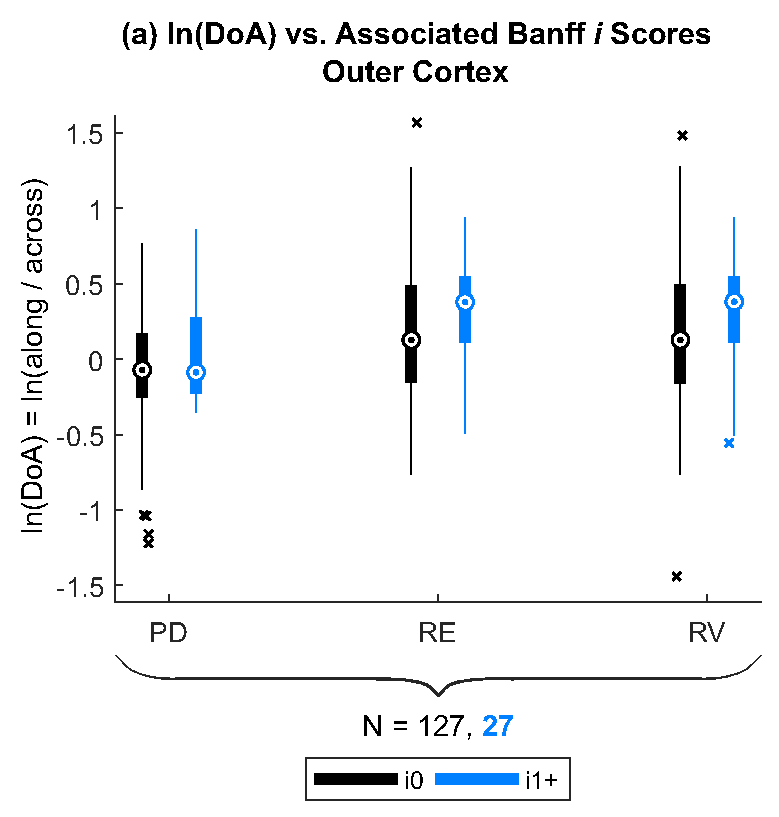
\includegraphics[width=0.24\textwidth]{
            parts/transplant/figs/boxplot-doa/doa-all-i/doa_F1.5_i_oc.eps
        }
        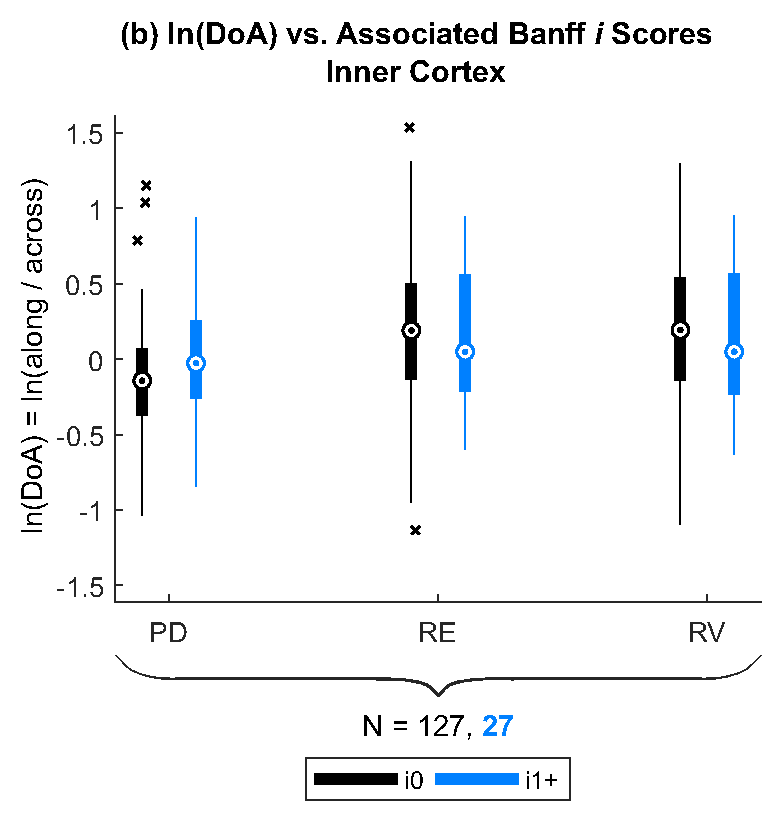
\includegraphics[width=0.24\textwidth]{
            parts/transplant/figs/boxplot-doa/doa-all-i/doa_F1.5_i_ic.eps
        }
        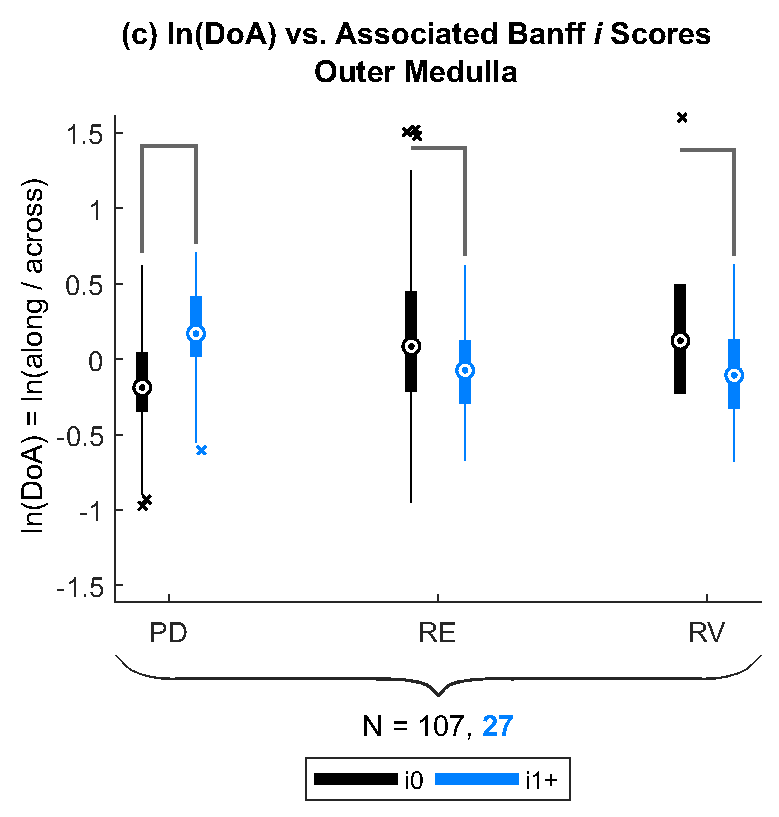
\includegraphics[width=0.24\textwidth]{
            parts/transplant/figs/boxplot-doa/doa-all-i/doa_F1.5_i_om.eps
        }
        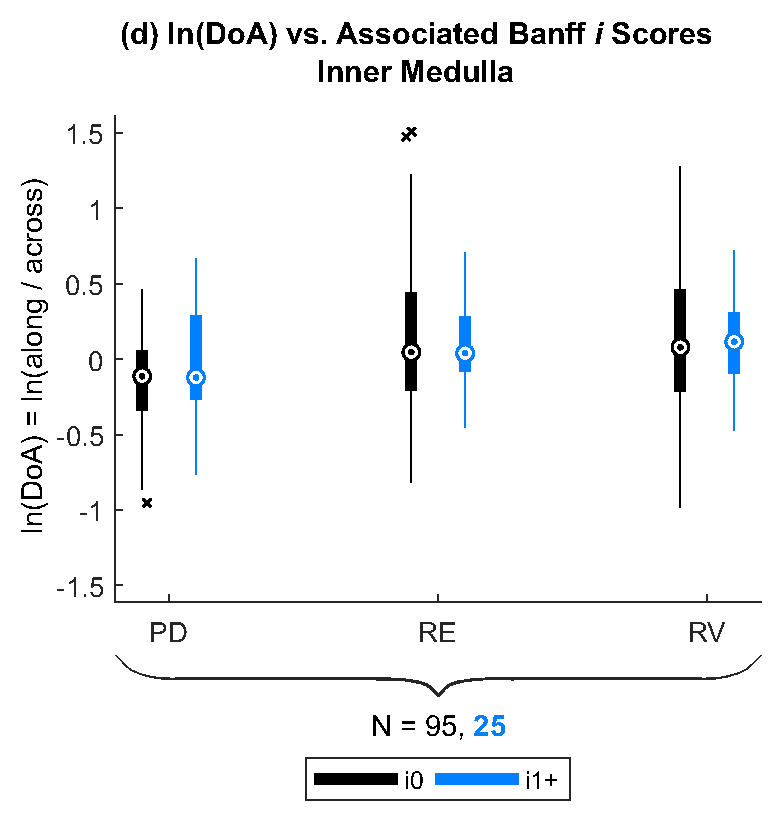
\includegraphics[width=0.24\textwidth]{
            parts/transplant/figs/boxplot-doa/doa-all-i/doa_F1.5_i_im.eps
        }
    \end{subfigure}
    \begin{subfigure}[b]{\textwidth}
        \centering
        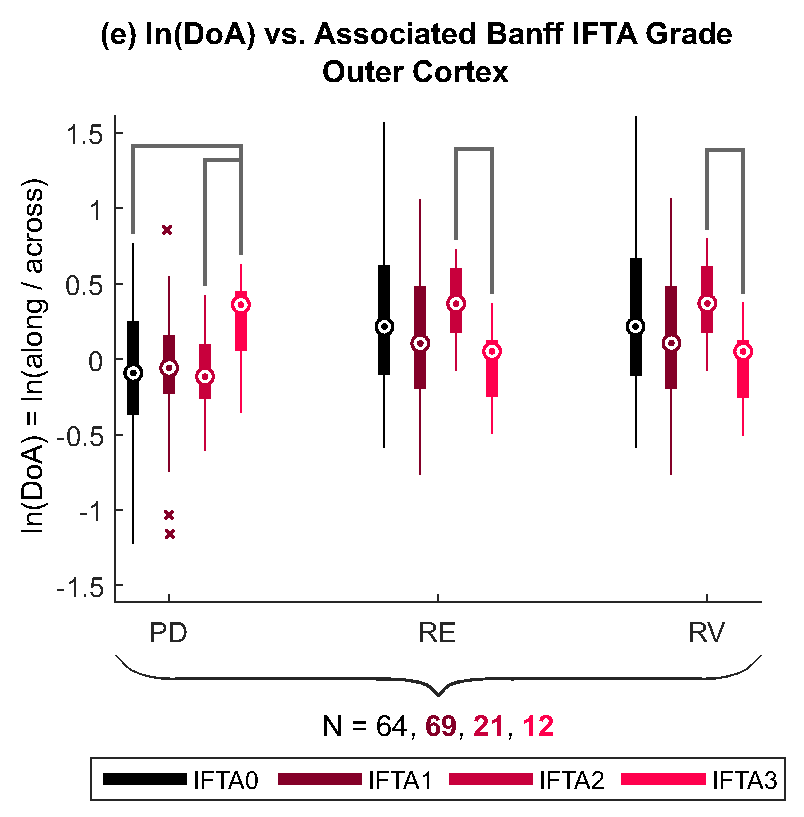
\includegraphics[width=0.24\textwidth]{
            parts/transplant/figs/boxplot-doa/doa-all-ifta/doa_F1.5_ifta_oc.eps
        }
        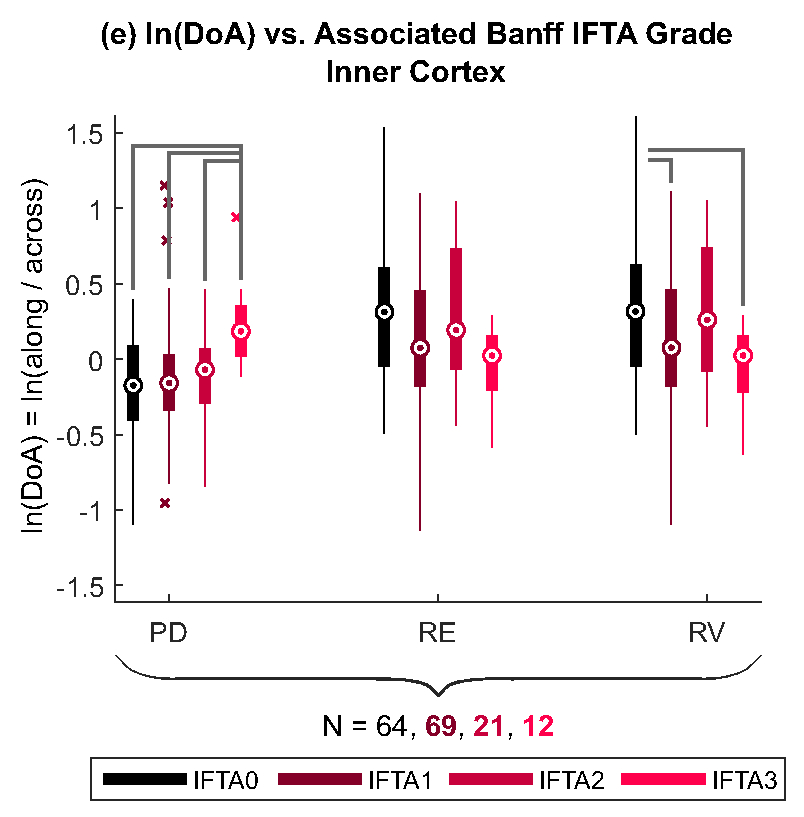
\includegraphics[width=0.24\textwidth]{
            parts/transplant/figs/boxplot-doa/doa-all-ifta/doa_F1.5_ifta_ic.eps
        }
        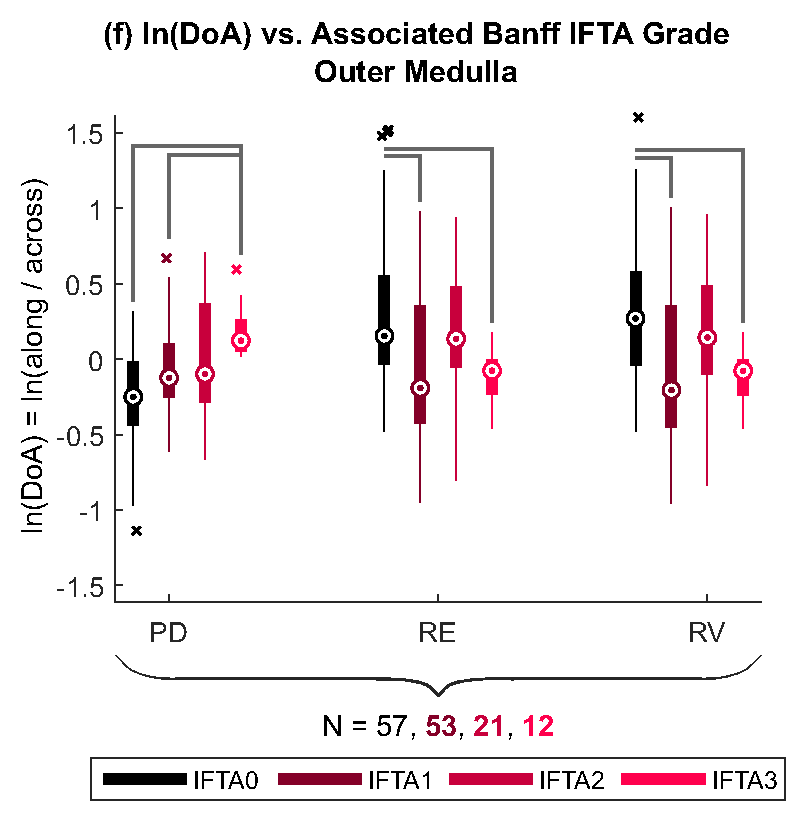
\includegraphics[width=0.24\textwidth]{
            parts/transplant/figs/boxplot-doa/doa-all-ifta/doa_F1.5_ifta_om.eps
        }
        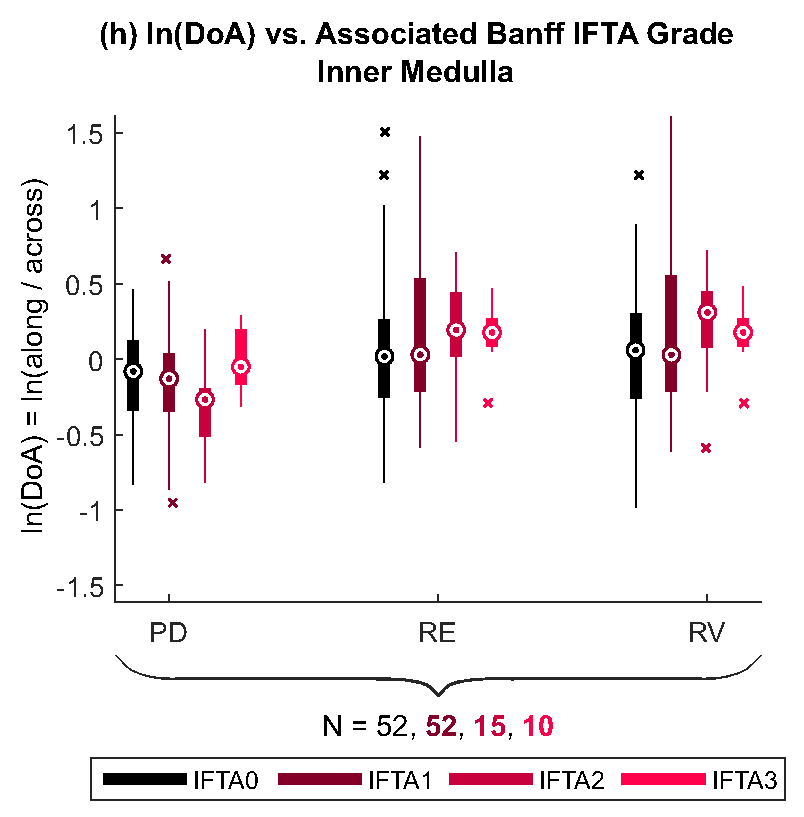
\includegraphics[width=0.24\textwidth]{
            parts/transplant/figs/boxplot-doa/doa-all-ifta/doa_F1.5_ifta_im.eps
        }
    \end{subfigure}
    \begin{subfigure}[b]{\textwidth}
        \centering
        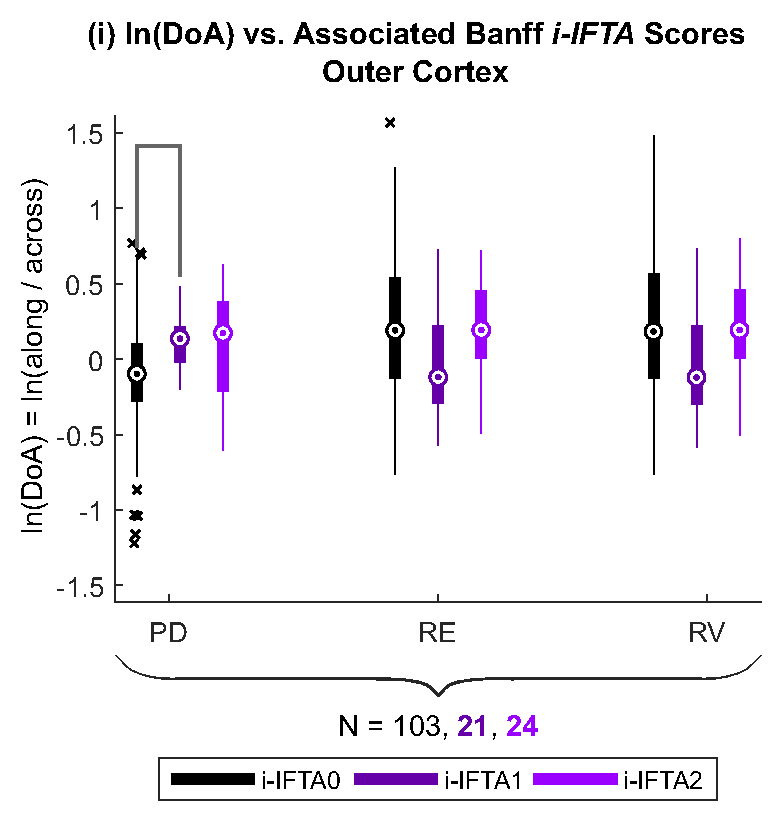
\includegraphics[width=0.24\textwidth]{
            parts/transplant/figs/boxplot-doa/doa-all-i-ifta/doa_F1.5_i-ifta_oc.eps
        }
        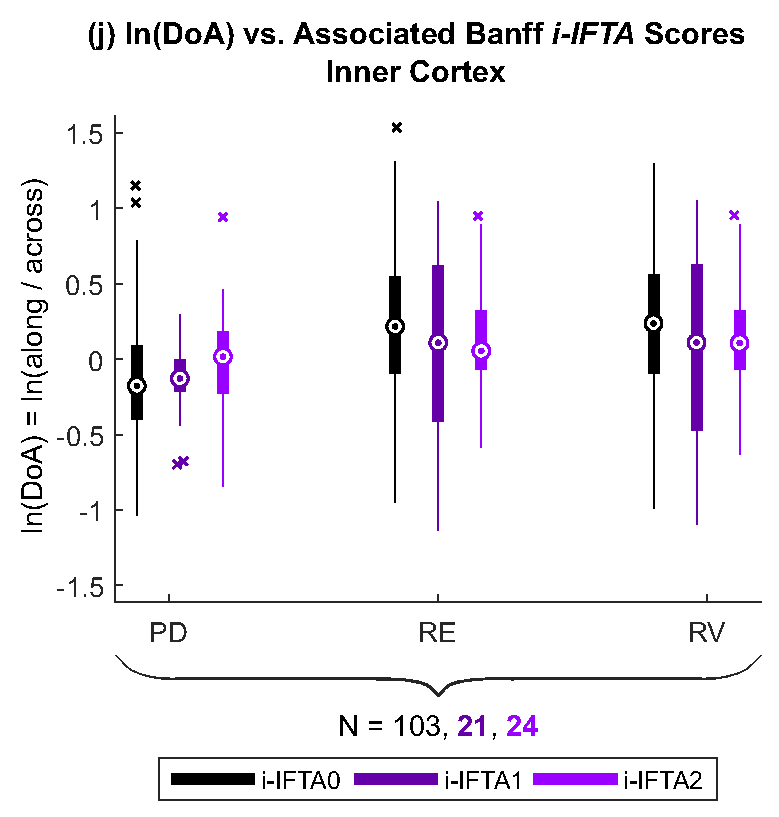
\includegraphics[width=0.24\textwidth]{
            parts/transplant/figs/boxplot-doa/doa-all-i-ifta/doa_F1.5_i-ifta_ic.eps
        }
        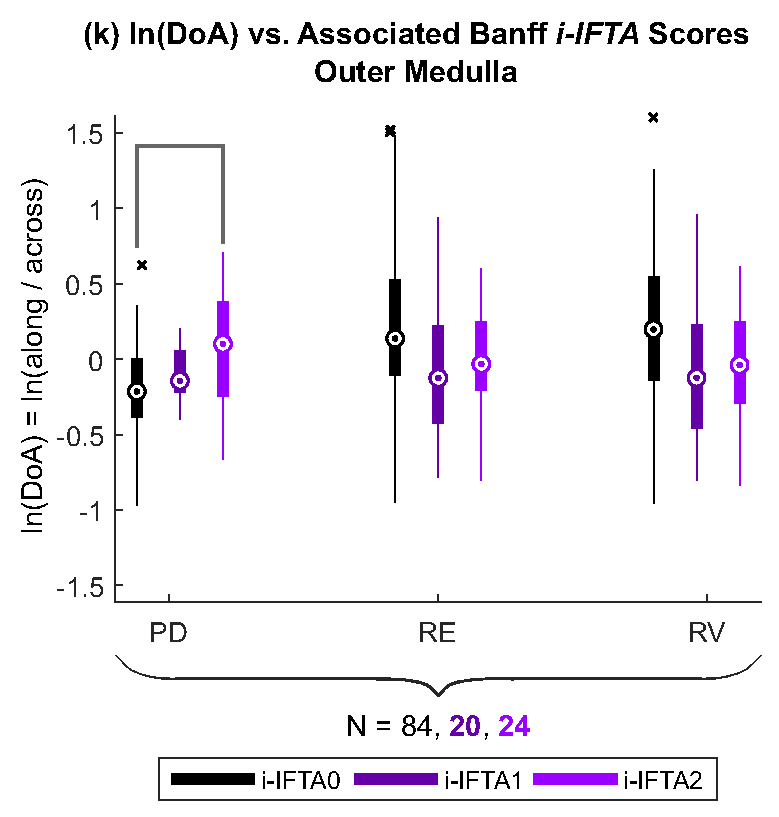
\includegraphics[width=0.24\textwidth]{
            parts/transplant/figs/boxplot-doa/doa-all-i-ifta/doa_F1.5_i-ifta_om.eps
        }
        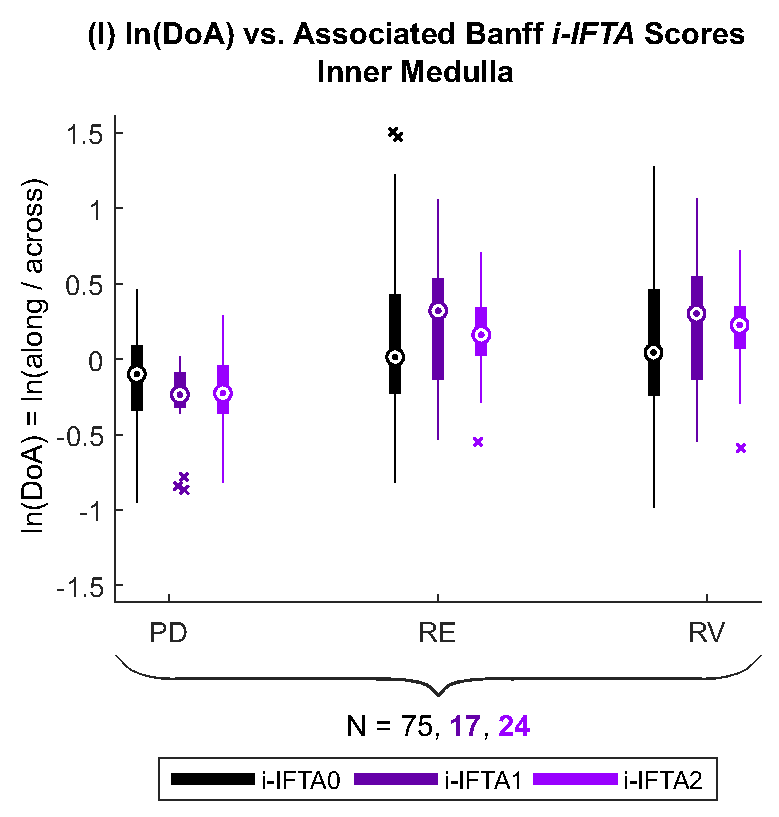
\includegraphics[width=0.24\textwidth]{
            parts/transplant/figs/boxplot-doa/doa-all-i-ifta/doa_F1.5_i-ifta_im.eps
        }
    \end{subfigure}
    \begin{subfigure}[b]{\textwidth}
        \centering
        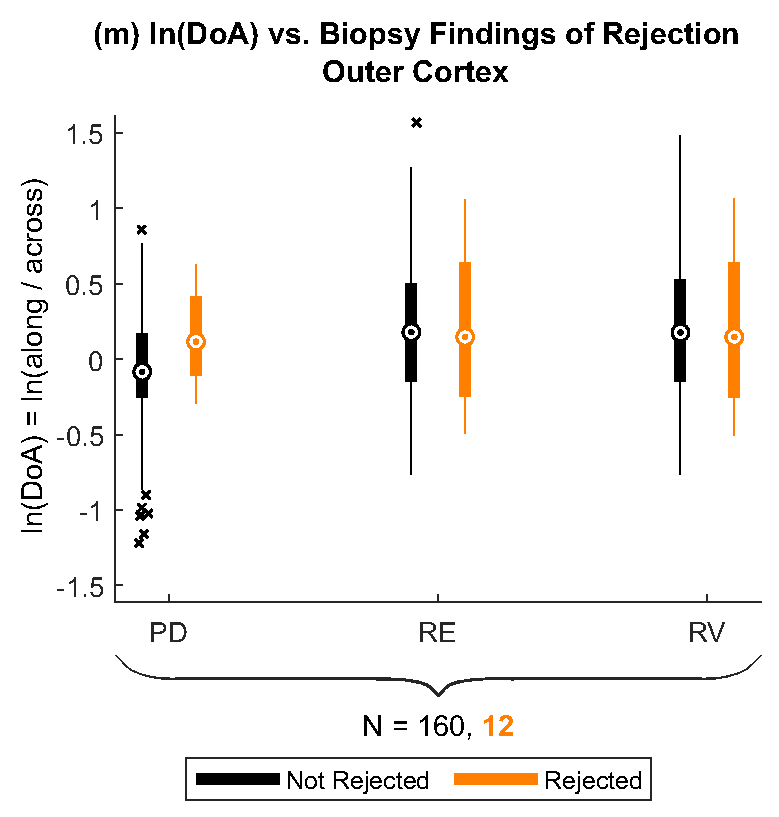
\includegraphics[width=0.24\textwidth]{
            parts/transplant/figs/boxplot-doa/doa-all-reject/doa_F1.5_reject_oc.eps
        }
        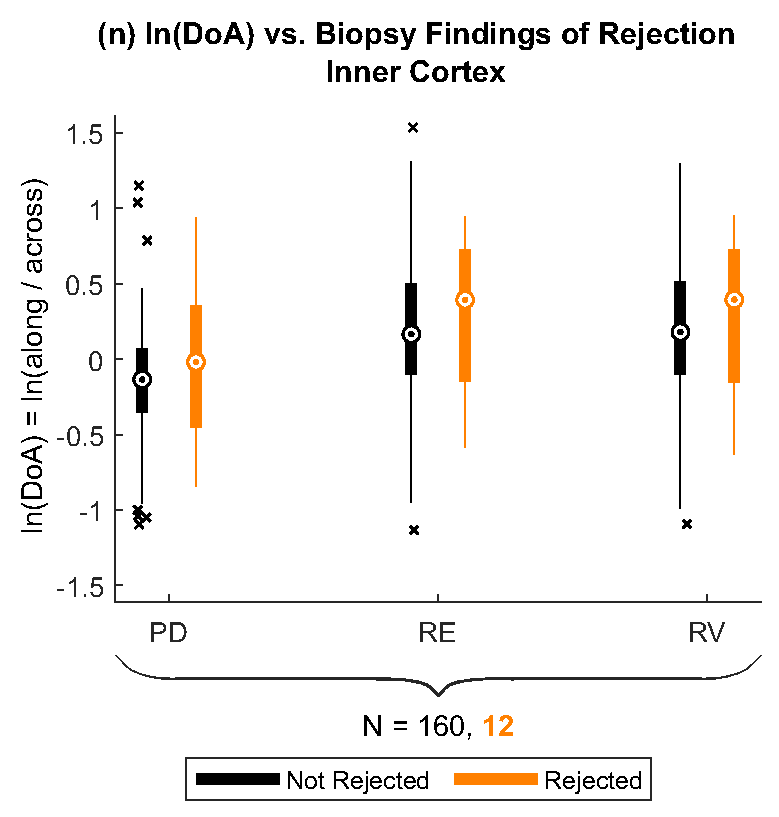
\includegraphics[width=0.24\textwidth]{
            parts/transplant/figs/boxplot-doa/doa-all-reject/doa_F1.5_reject_ic.eps
        }
        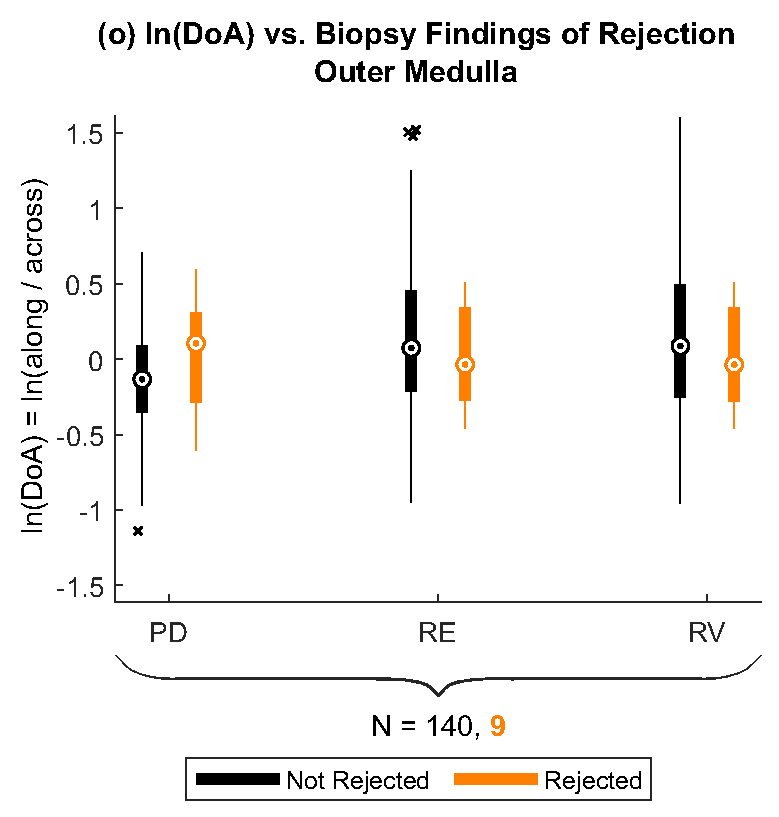
\includegraphics[width=0.24\textwidth]{
            parts/transplant/figs/boxplot-doa/doa-all-reject/doa_F1.5_reject_om.eps
        }
        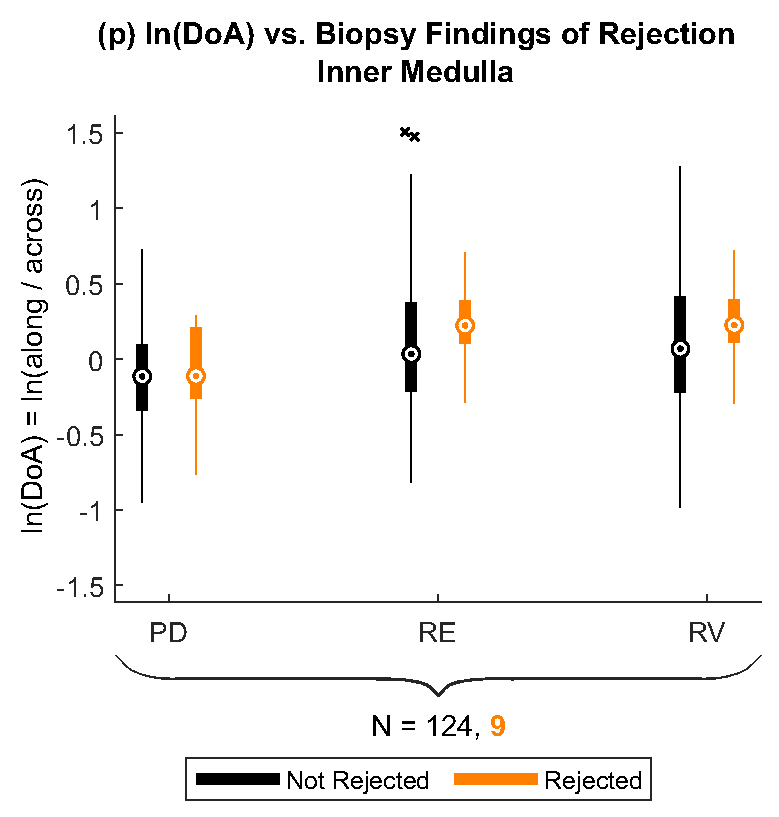
\includegraphics[width=0.24\textwidth]{
            parts/transplant/figs/boxplot-doa/doa-all-reject/doa_F1.5_reject_im.eps
        }
    \end{subfigure}
    \caption{Box plots of DoA based on PD, RE, and RV measurements, grouped by associated biopsy findings of (a--d) \emph{i} (interstitial inflammation) scores, (e--h) IFTA (interstitial fibrosis/tubular atrophy) grading, (i--l) \emph{i-IFTA} (inflammation in areas of IFTA) scores, and (m--p) whether biopsies indicated graft rejection. Values are shown for DoA at the (a,e,i,m) outer cortex, (b,f,j,n) inner cortex, (c,g,k,o) outer medulla, and (d,h,l,p) inner medulla. Numbers written under x-axes denote number of ROIs represented by each distribution. Pairs of box plots connected with gray bars denote statistically significant differences ($p < 0.05$) between biopsy findings based on Kruskal-Wallis test and Bonferroni correction. DoA values without matched biopsy findings are not shown.}
    \label{fig:clinicalVisrDoa}
\end{figure}
